\documentclass[tikz]{standalone}
\usepackage{pgfplots}
\pgfplotsset{compat=1.15}
\usepackage{mathrsfs}
\usetikzlibrary{arrows,calc}
\usepackage{tkz-euclide}
\pagestyle{empty}

\definecolor{AngleClr}{rgb}{0,0.39215686274509803,0}
\definecolor{ShapeClr}{rgb}{0.6,0.2,0}

\begin{document}

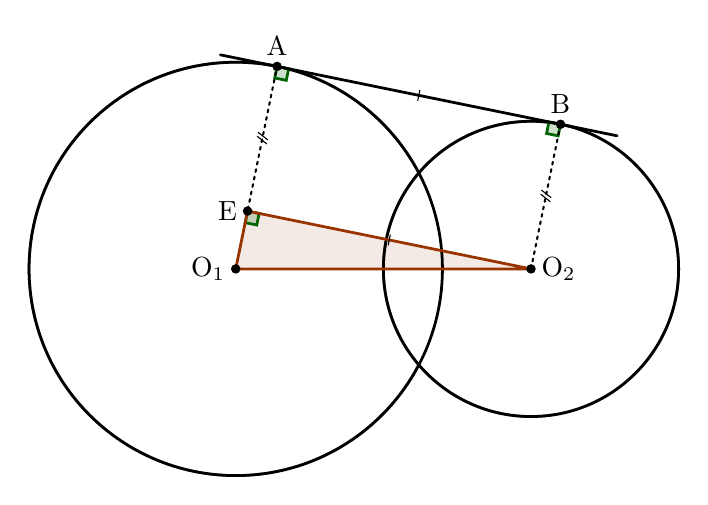
\begin{tikzpicture}[scale=.75]
\tkzSetUpLine[line width=1pt,color=black]
\tkzSetUpPoint[fill=black]

\tkzDefPoints{0/0/O1,5/0/O2,3.5/0/A,2.5/0/B,17.5/0/P}

\tkzDefTangent[from = P](O1,A) \tkzGetPoints{TC}{TA}
\tkzDefTangent[from = P](O2,B) \tkzGetPoints{TD}{TB}

\tkzDefPointBy[projection=onto O1--TA](O2) \tkzGetPoint{E}

\tkzDrawCircle[line width=1.0pt,fill=white](O1,A)
\tkzDrawCircle[line width=1.0pt,fill=white](O2,B)

\tkzFillPolygon[fill=ShapeClr,fill opacity=0.1](O1,E,O2)

\tkzDrawCircle[line width=1.0pt,color=black](O1,A)
\tkzDrawCircle[line width=1.0pt,color=black](O2,B)

\tkzInterCC(O1,A)(O2,B) \tkzGetPoints{C}{D}
\tkzInterLL(O1,O2)(C,D) \tkzGetPoint{X}

\tkzMarkRightAngles[line width=1pt, size=.2,color=AngleClr,fill=AngleClr,fill opacity=0.2](O1,TA,TB O2,TB,TA O1,E,O2)

% \tkzDrawSegments[line width=1pt,color=black](O1,O2 C,D)
\tkzDrawSegments[line width=1pt,color=black,add=0.2 and 0.2](TA,TB)
\tkzDrawSegments[line width=0.75pt,color=black,dashed,dash pattern=on 1pt off 1.75pt](O1,TA O2,TB)
\tkzDrawPolygon[color=ShapeClr](O1,E,O2)


\tkzDrawPoints[size=3](O1,O2,TA,TB,E)
\tkzLabelPoint[left](O1){$\rm O_1$}
\tkzLabelPoint[right](O2){$\rm O_2$}
\tkzLabelPoint[above](TA){$\rm A$}
\tkzLabelPoint[above](TB){$\rm B$}
\tkzLabelPoint[left](E){$\rm E$}

\tkzMarkSegments[mark=|,size=2](TA,TB E,O2)
\tkzMarkSegments[mark=s||,size=2](E,TA O2,TB)

\end{tikzpicture}
\end{document}

